\documentclass[11pt]{article}

\usepackage[left=1in, right=1in, top=1in, bottom=1in, paperwidth=8.5in, paperheight=35in]{geometry} % Adjust 'paperheight' as needed

\usepackage{graphics,epsfig,graphicx,float,subfigure,color}
\usepackage{algorithm,algorithmic}
\usepackage{amsmath,amssymb,amsbsy,amsfonts,amsthm}
\usepackage[small,bf,up]{caption}


\usepackage{soul}
\usepackage{comment}
\usepackage{url}
\usepackage{boxedminipage}
\usepackage[sf,bf,small]{titlesec}
\usepackage[textsize=footnotesize]{todonotes}
\usepackage[plainpages=false, colorlinks=true,
   citecolor=blue, filecolor=blue, linkcolor=blue,
   urlcolor=blue]{hyperref}

\usepackage{amsmath}

\include{ogmacros}

\newcommand{\bdm}{\begin{displaymath}}
\newcommand{\edm}{\end{displaymath}}

\newcommand{\ben}{\begin{enumerate}}
\newcommand{\een}{\end{enumerate}}

\newcommand{\p}{\partial}
\newcommand{\bs}{\boldsymbol}

\usepackage{amssymb}

%$\mathbb{R}$

\parskip 1ex

\parindent 0ex

\begin{document}
\pagestyle{empty}

\begin{center}
{\large {\bf MATH 140: Mathematical Methods for Optimization}}\\
{\bf Assignment 6---Spring 2024}\\
{\bf Due March 14, 2024} \\
{\textcolor{red}{\bf By:Ronald Nap}}

\end{center}

\begin{enumerate}

\item (\textbf{5 points}) Recall that rank-one matrices are matrices that have only one linearly independent column, i.e., every column is a multiple of each other. Also, note that every rank-one matrix $U$ can be written as the \textsl{outer product} $U = uv^T$, where $u$ and $v$ are column vectors.
\begin{enumerate}
    \item Let $B$ be a symmetric positive definite matrix and let $U$ be a symmetric rank-one matrix. To show that $B+U$ is positive definite, 
    \begin{enumerate}
        \item[\textcolor{red}{Solution:}] 
        \textcolor{red}{Since $B$ is positive definite, we have $x^TBx > 0$.} 
        \textcolor{red}{Given $U$ is a rank-one symmetric matrix, it can be expressed as $U = uv^T$ for some column vectors $u$ and $v$.} 
        \textcolor{red}{Therefore, $x^TUx = x^Tuv^Tx = (v^Tx)(u^Tx)$.} 
        \textcolor{red}{The product $(v^Tx)(u^Tx)$ is a scalar and can be non-negative.} 
        \textcolor{red}{Therefore, for any nonzero vector $x$, it follows that $x^T(B+U)x = x^TBx + x^TUx > 0$,} 
        \textcolor{red}{proving that $B+U$ is positive definite.}
    \end{enumerate}

    \item Suppose $A$ and $B$ are both symmetric positive definite.
    Show that $A+B$ is also symmetric positive definite.
    
\begin{enumerate}
    \item[\textcolor{red}{Solution:}] 
    \textcolor{red}{Since $A$ is symmetric positive definite, for any nonzero $x$, we have $x^TAx > 0$.}
    \textcolor{red}{Similarly, because $B$ is also symmetric positive definite, for the same nonzero $x$, $x^TBx > 0$.}
    \textcolor{red}{Adding these two inequalities yields $x^TAx + x^TBx > 0 + 0$, which simplifies to $x^T(A+B)x > 0$.}
    \textcolor{red}{This inequality demonstrates that $A+B$ is positive definite for any nonzero vector $x$.}
    \textcolor{red}{Therefore, $A+B$ is symmetric positive definite.}
\end{enumerate}

\end{enumerate}





  
  \item ({\bf 5 points}) Recall that the Symmetric Rank-1 (SR1) update
    is given by the following:
  $$B_{k+1} = B_k + \underbrace{\frac{1}{(y_k - B_ks_k)^Ts_k}(y_k
    -B_ks_k)(y_k- B_ks_k)^T}_{U_k},$$ where $s_k = x_{k+1}-x_{k}$ and
  $y_k = \nabla f_{k+1} - \nabla f_k$. Note that the update matrix
  $U_k$ is symmetric and has rank one.

  
  \begin{enumerate}
  \item Show that $B_{k+1}$ satisfies the secant condition $B_{k+1} s_k = y_k$.


\begin{enumerate}
    \item[\textcolor{red}{Solution:}] 
    \textcolor{red}{Recall:}
    \textcolor{red}{
    \[
    B_{k+1} = B_k + \frac{(y_k - B_ks_k)(y_k - B_ks_k)^T}{(y_k - B_ks_k)^Ts_k}
    \]
    }
    \textcolor{red}{Lets multiply both sides by \(s_k\):}
    \textcolor{red}{
    \[
    B_{k+1}s_k = (B_k + \frac{(y_k - B_ks_k)(y_k - B_ks_k)^T}{(y_k - B_ks_k)^Ts_k})s_k
    \]
    }
    \textcolor{red}{Expanding the RHS:}
    \textcolor{red}{
    \[
    = B_ks_k + \frac{(y_k - B_ks_k)(y_k - B_ks_k)^Ts_k}{(y_k - B_ks_k)^Ts_k}
    \]
    }
    \textcolor{red}{Cancel Out:}
    \textcolor{red}{
    \[
    = B_ks_k + (y_k - B_ks_k) = y_k
    \]
    }
    \textcolor{red}{Therefore, \(B_{k+1}s_k = y_k\).}
\end{enumerate}



  
  \item Show that the inverse of $B_{k+1}$ is given by
    $$ B_{k+1}^{-1} = B_k^{-1} + \frac{1}{(s_k - B_k^{-1}y_k)^Ty_k}(s_k -
    B_k^{-1}y_k)(s_k - B_k^{-1}y_k)^T.
    $$

\begin{enumerate}
    \item[\textcolor{red}{Solution:}] 
    \textcolor{red}{Recall Sherman-Morrison formula, if \(A\) is invertible and \(uv^T\) is a rank-one update, then:}
    \textcolor{red}{
    \[
    (A + uv^T)^{-1} = A^{-1} - \frac{A^{-1}uv^TA^{-1}}{1 + v^TA^{-1}u}
    \]
    }
    \textcolor{red}{For the SR1 update, we substitute \(A = B_k\), \(u = s_k - B_k^{-1}y_k\), and \(v^T = (s_k - B_k^{-1}y_k)^T\), this means \(B_{k+1} = B_k + U_k\) where \(U_k\) is the rank-one update matrix.}
    \textcolor{red}{
    \[
    B_{k+1}^{-1} = B_k^{-1} - \frac{B_k^{-1}(s_k - B_k^{-1}y_k)(s_k - B_k^{-1}y_k)^TB_k^{-1}}{1 + (s_k - B_k^{-1}y_k)^TB_k^{-1}(s_k - B_k^{-1}y_k)}
    \]
    }
    \textcolor{red}{We can observe that \(y_k = B_{k+1}s_k - B_ks_k\) by the secant condition, simplifying the expression for \(B_{k+1}^{-1}\) inversely relates to the direct SR1 update through the inverse properties of \(B_k\) and \(B_{k+1}\).}
    \textcolor{red}{This confirms the inverse formula aligning with the properties of matrix inverses and the SR1 update mechanism.}
\end{enumerate}


    
  \end{enumerate}




  
 \item (Matlab, {\bf 10 points}) Consider the unconstrained
  optimization problem
  \begin{align}
  \min f(x,y) \equiv - \cos x \cos (y/10)
  \end{align}
  from the fourth and fifth homework assignments.
  
  \begin{enumerate}
  
  \item Change your Newton implementation (written for hw5) to perform
    quasi-Newton (BFGS) iterations with line search. Note, for the
    BFGS method you will need to use the Wolfe condition given in
    class (see equations 3.6a and 3.6b in Nocedal \& Wright's
    book). You can start with $\alpha_0 = 1$ as the initial trial step
    length.



    \begin{figure}[H]
    \centering
    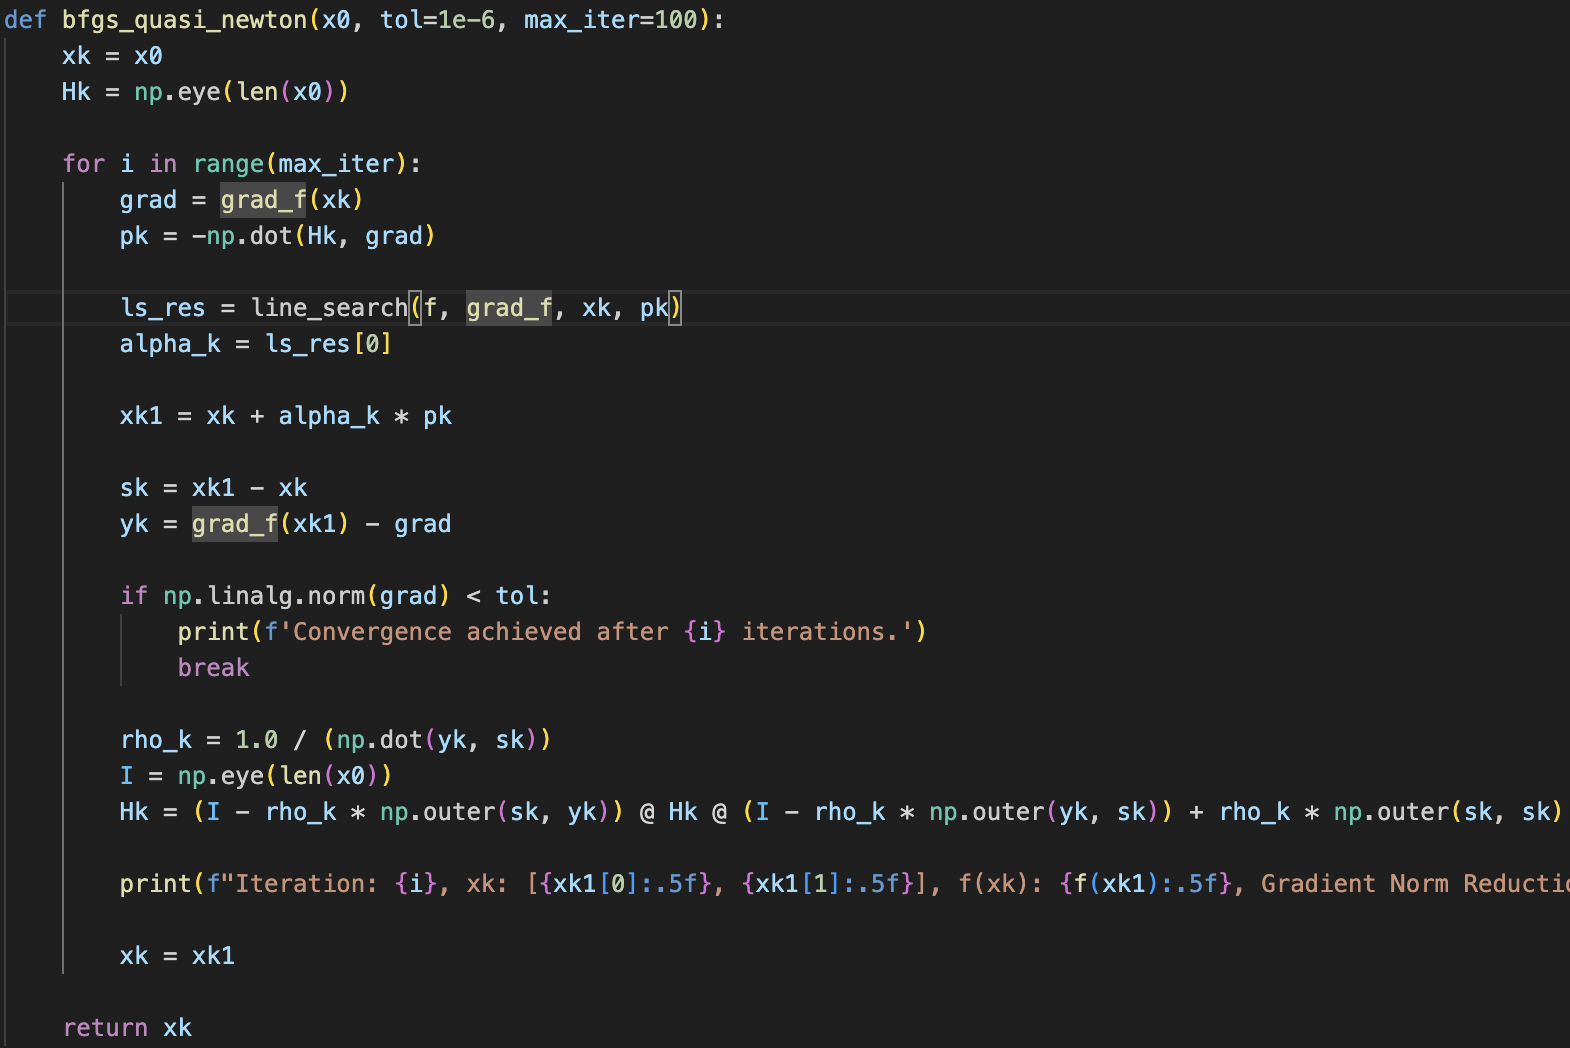
\includegraphics[width=\textwidth]{3a.png} 
    \end{figure}

    
  \item Run your program for various initial guesses within the region
    where you found the Hessian to be positive definite (see hw4).  At
    every iteration print out the iteration, the current point $x_k$,
    the value of the objective function $f(x_k)$, and the reduction in
    the norm of the gradient $ \|\nabla f(x_k)\|_2/ \|\nabla
    f(x_0)\|_2$.

    \begin{figure}[H]
    \centering
    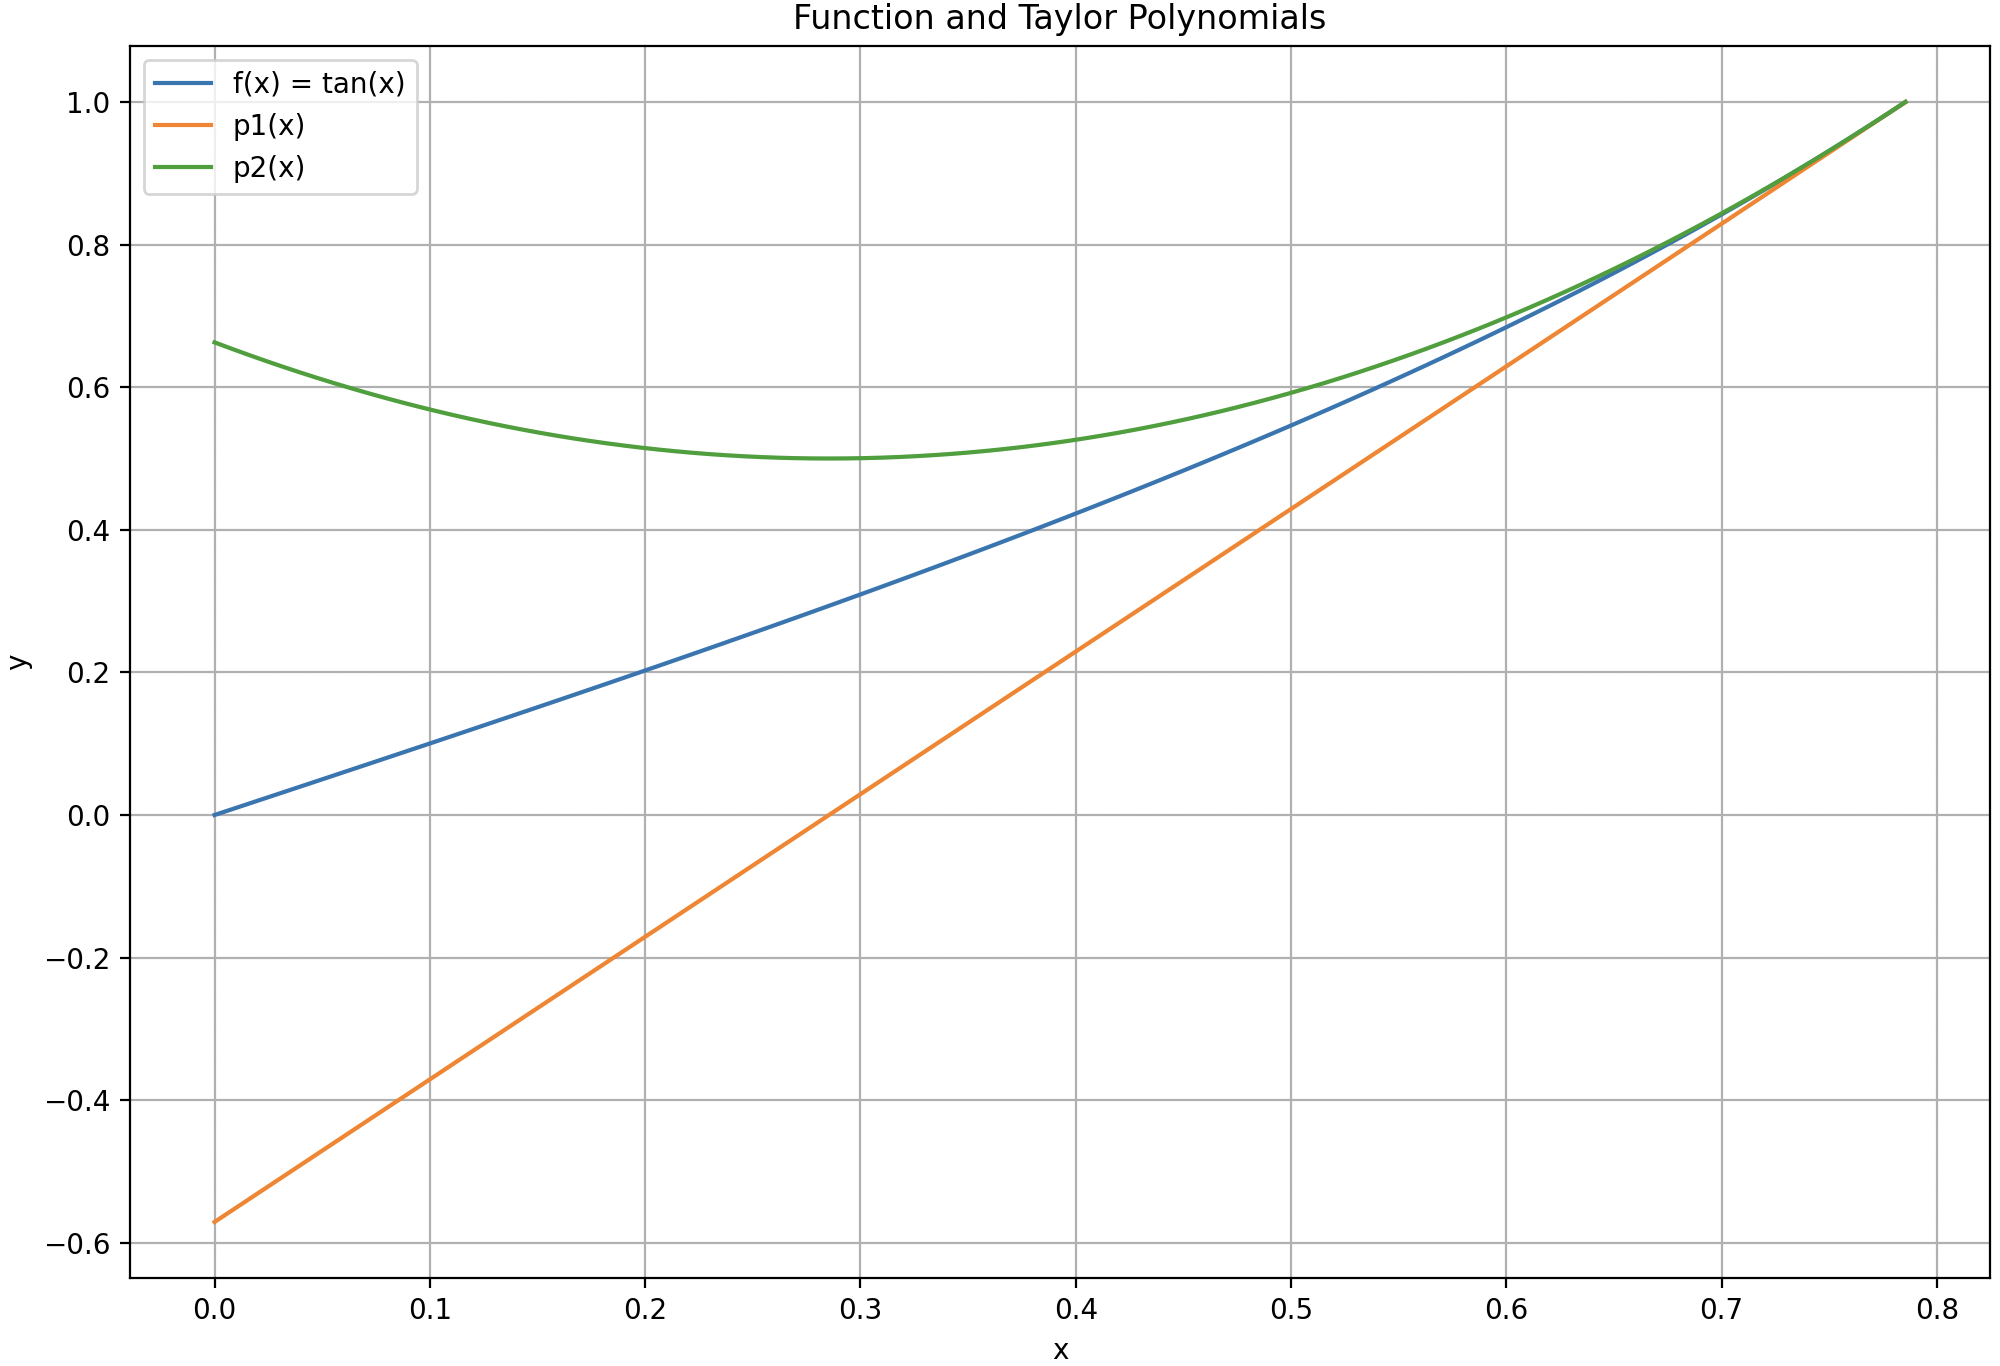
\includegraphics[width=\textwidth]{3b.png} 
    \end{figure}

    
  \item What do you observe about the convergence rate for this
    method? How does BFGS compare to Newton's method.

\item[\textcolor{red}{Solution:}] 
\textcolor{red}{
The results indicate Newton's method demonstrates a faster convergence rate compared to the BFGS method, reaching convergence within 3 to 4 iterations as opposed to 11 iterations required by BFGS. This is expected since Newton has quadratic convergence which is typically faster. For both methods, the step size remains at 1.0 throughout the iterations. This suggests that the initial search direction is efficient and there is no need to adjust it. Both methods converge to [0,0] across various initial guesses suggesting that [0,0] is the global minimum for the function within the domain. The Gradient Norm Reduction approaches zero confirming that both methods are successfully converging in on a point where the gradient is negligible. While Newton's method is quicker in iteration count, it also has a higher computational cost per iteration due to the calculation and inversion of the Hessian matrix, as opposed to the BFGS method, which approximates the Hessian.
}









    
  \end{enumerate}

    \end{enumerate}
\end{document}
